\section{Fulfillment of Requirements}\label{sc:discRequirement}
In order to evaluate the system, it is important to look at how well it fulfills the requirements set for it in cooperation with the client. In \autoref{fig:discRequirements} the requirements have been colored according to whether they have been fulfilled or not. Green indicates a fulfilled requirement, yellow a partially fulfilled one, and red a requirement that has not been fulfilled.  
%overordnet om dem der er fullfilled (unit tests)




\begin{figure}[H]
    \centering
    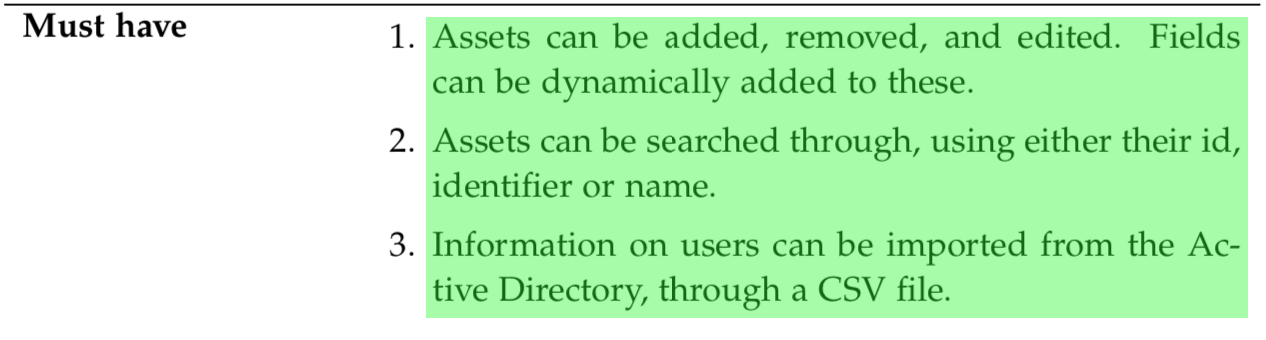
\includegraphics[width=0.9\textwidth]{figures/Requirements/MustHave.png}
\end{figure}
\vspace{-10mm}
\begin{figure}[H]
    \centering
    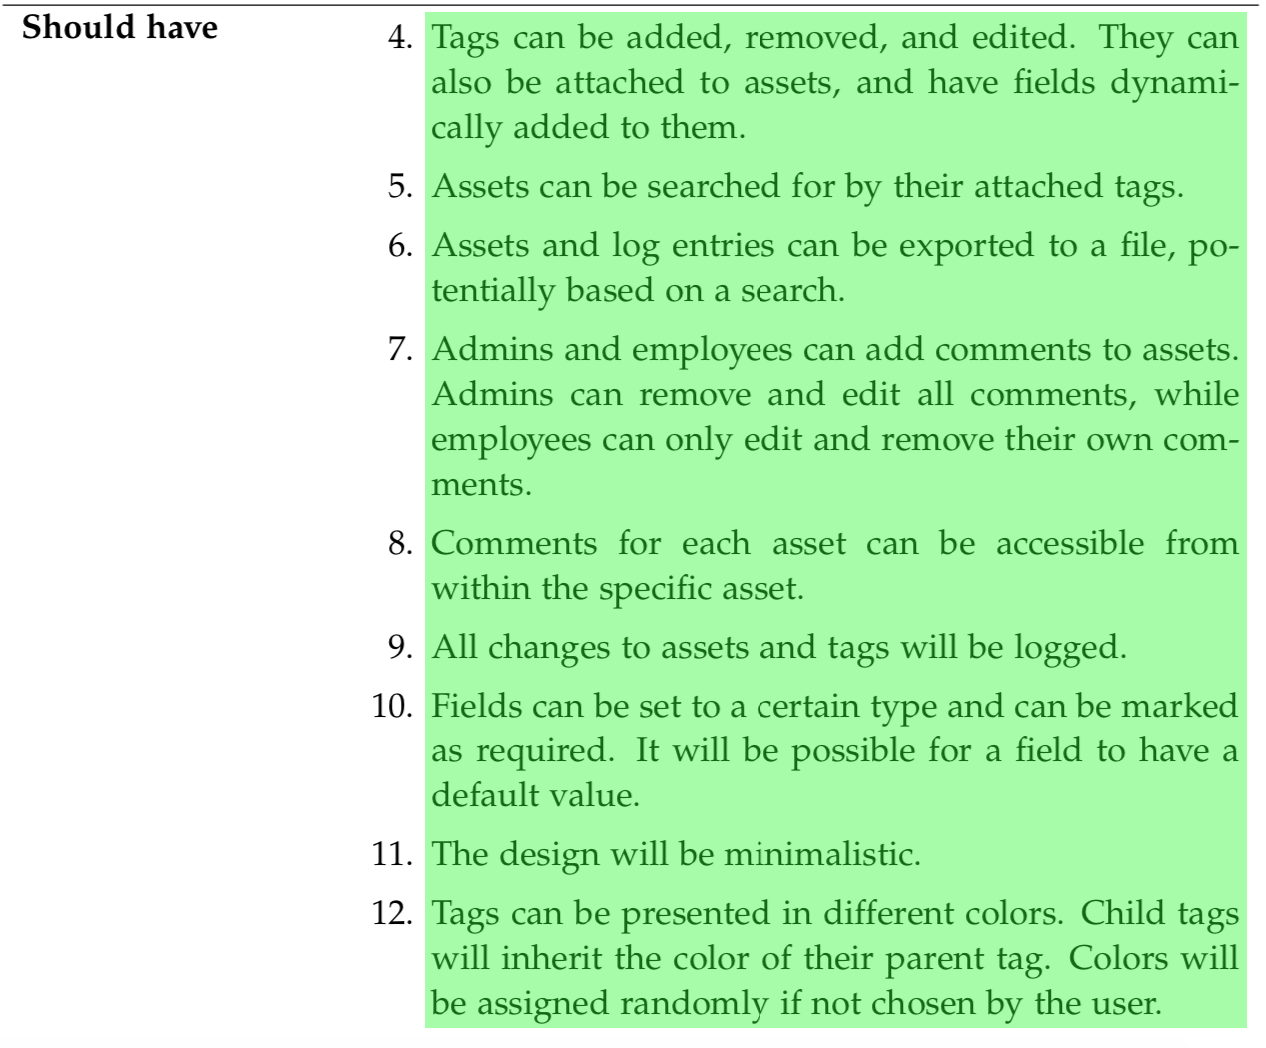
\includegraphics[width=0.9\textwidth]{figures/Requirements/ShouldHave.png}
\end{figure}
\vspace{-10mm}
\begin{figure}[H]
    \centering
    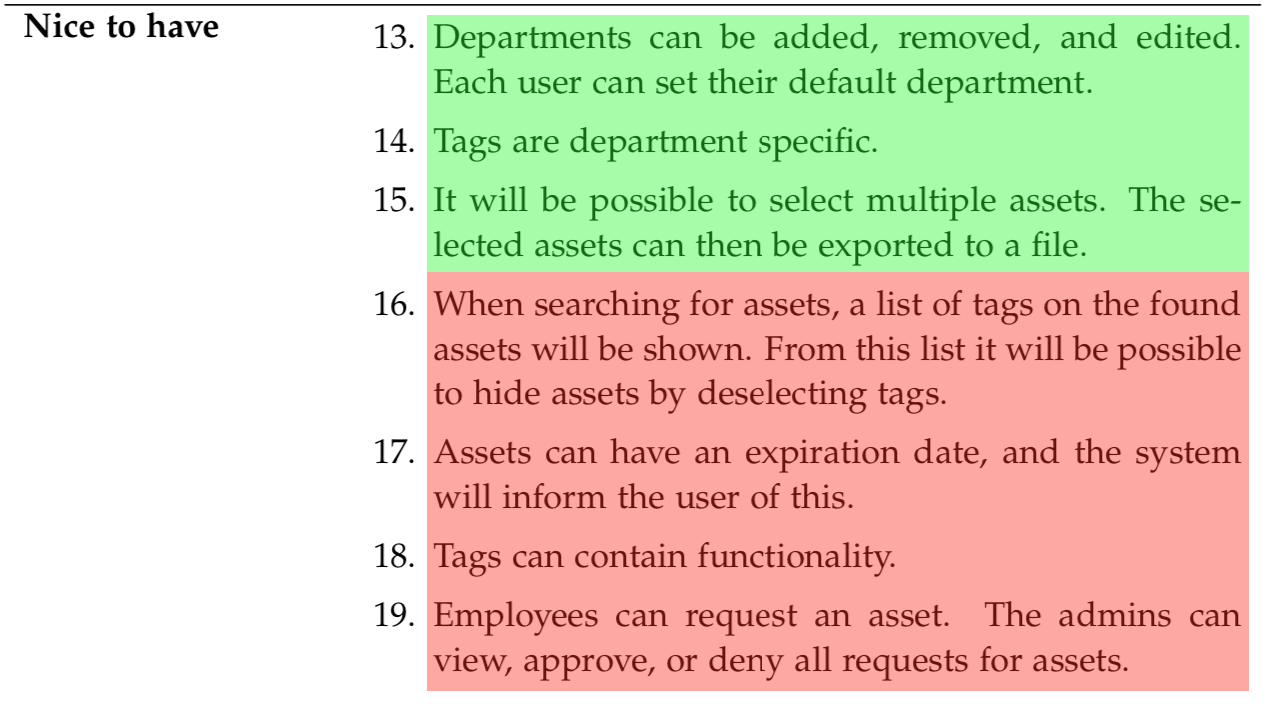
\includegraphics[width=0.9\textwidth]{figures/Requirements/NiceToHave.png}
\end{figure}
\vspace{-10mm}
\begin{figure}[H]
    \centering
    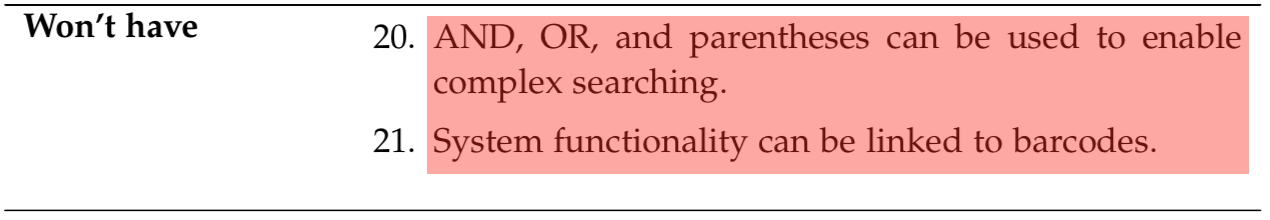
\includegraphics[width=0.9\textwidth]{figures/Requirements/WontHave.png}
    \caption{Table indicating how well the requirements have been fulfilled. Green indicates a fulfilled requirement and red a requirement that has not been fulfilled }
    \label{fig:discRequirements}
\end{figure}

All the \textit{Must have} requirements have been fulfilled as well as all of the \textit{Should have} requirements. This has been confirmed through unit and usability tests.
%\par
%Requirement 7 is only partially fulfilled. This requirement states that the admins and employees should be able to add, edit and remove comments. It is, however, not possible to edit any comments in the system. This part of the requirement has, after further discussion with the client, been deemed less important than other functionalities, such as logging changes made to assets and tags.
\par
Requirement 11 is difficult to evaluate as it is vague and subjective. It has been judged as fulfilled based on \citep{MinimalistUX}. For instance the UI has been designed to look flat, the menus are simple and visible, and UI elements are limited to the most necessary ones. This is in accordance with the guidelines given by \citep{MinimalistUX}.
\par
The requirements not fulfilled, have had a lower priority than the ones implemented in the system. As seen in \autoref{fig:discRequirements}, functionalities meeting the requirements have been implemented in a prioritized manner. This means that the first requirement was implemented before the second and so on.